 %%
%%
%%   This file is based on the ``apstemplate.tex'' from
%%   the APS files in the REVTeX 4 distribution.
%%   Version 4.1r of REVTeX, August 2010
%%   See the REVTeX 4 README file for restrictions and more information.
%%
%
% This is a template for producing manuscripts for use in PHYS3605 at
% the University of Minnesota
%
% Copy this file to another name and then work on that file.
% That way, you always have this original template file to use.

\documentclass[aps,prstab,reprint,12pt]{revtex4-1}
\usepackage[title]{appendix}
\usepackage{xspace}
\usepackage{amsfonts}
\usepackage{graphicx}
\usepackage{siunitx}
\usepackage{grffile}
\usepackage{float}
\usepackage{mathrsfs}

\usepackage[utf8]{inputenc}

\usepackage[letterpaper, margin=0.8in]{geometry}



\providecommand{\units}[1]{\,\ensuremath{\mathrm{#1}}\xspace}


\newcommand{\appendixpdf}[3]{
    \includepdf[pages=1,scale=.8,pagecommand={\section{#1}\label{#3}},linktodoc=true]{#2}
    \includepdf[pages=2-,scale=.8,pagecommand={\section*{Appendix \ref{#3}\quad #1}},linktodoc=true]{#2}
}

% \linespread{2}

\begin{document}

%Title of paper
\title{A Relation of Mechanical and Electrical Power using a Watt Balance}

% Your name should go first, marked as ``communicating author'' 
\author{M. Laraia and J. Hirschi}
% Your lab partner or partners can come next

\affiliation{University of Minnesota, Minneapolis, MN, USA}

\date{\today}

\begin{abstract}
    % We propose to construct a watt balance for the purpose of balancing mechanical power and electrical power. The work done by Chao et al. at the National Institute of Standards and Technology in the construction of a Lego based watt balance will be replicated. We intend to improve the previous design after successful replication of unity measurements between mechanical and electrical power. 
    
    We describe the construction of a watt balance for the purpose of balancing mechanical and electrical power. Under the redefinition of SI units in 2019, the kilogram will be fixed to Planck's constant. The preferred method of realizing the kilogram from this new definition is using a Watt balance. We expect the Watt balance we construct to be capable of measuring the mass of an object to within 1\%.


    % As of 2018, the global effort to redefine our International System of Units (SI) has finished and the present base units of SI are now derived from fundamental constants of the universe. In particular, the unit of mass, the kilogram, is now realized through the fixed value of Plank's constant $h$. The National Institute of Standards and Technology (NIST) designed and constructed a "Watt Balance" to redefine the kilogram using $h$ to great precision. A LEGO Watt balance was constructed by NIST scientists for educational outreach and to demonstrate the principles of the Watt balance. Their design was capable of measuring a \si{gram} to 1\% relative uncertainty. We intend to recreate and improve upon their design through the use of different instruments and materials.
\end{abstract}

%\maketitle must follow title, authors, abstract
\maketitle

% body of paper here - Use proper section commands References should
% be done using the \cite, \ref, and \label commands
\section{INTRODUCTION}

Before 2018, the SI unit of mass was defined by the International Prototype Kilogram (IPK). The IPK was forged in 1879 out of a platinum-iridium alloy, and has been stored underground in Paris ever since. The mass of the IPK is fixed to $1\si{kg}$, and is the only mass in the world with zero uncertainty. This is problematic as it has been shown that the mass of the IPK has been drifting over the years when compared to its original copies. A definition of the kilogram based on a fixed object cannot be guaranteed to remain stable indefinitely over time.

\begin{figure}[h]
    \centering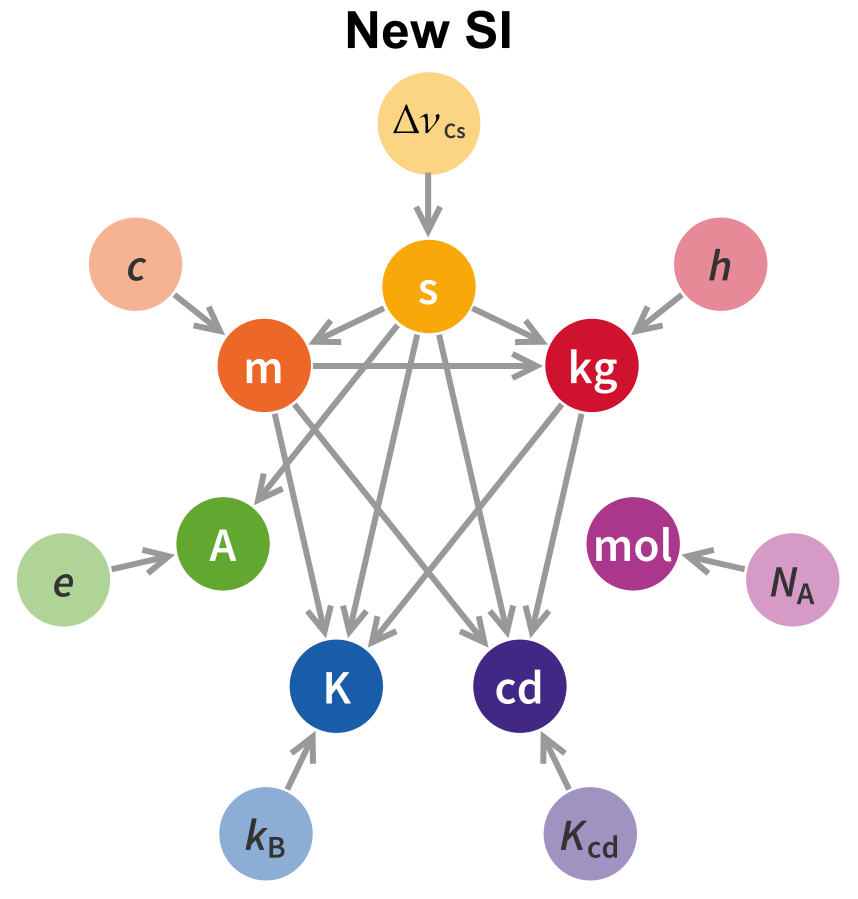
\includegraphics[width=.95\linewidth]{figs/si_units.png}
    \caption{As of May 20, 2019, all SI units will be defined in terms of fundamental constants of the universe. 
    % Notably, the units of kilogram, ampere, kelvin, and mole will be redefined in terms of Planck's constant $h$, the charge of an electron $e$, the Boltzmann constant $k$, and Avogagro's number $N_A$.
    \cite{wiki_si}}\label{fig:si}
\end{figure}

For this reason there is a push to redefine the SI units in terms of fundamental constants of the universe, as many of the original SI units were defined in a similar, sometimes arbitrary, way. For example, length has been redefined in terms of speed of light in vacuum, and time in terms of the period of radiation of a specific transition in caesium-133. The kilogram, ampere, kelvin, and mole are the last remaining SI units to be redefined in such terms. A summary of the fundamental dependencies of the redefined SI system is shown in figure \ref{fig:si}. 
%Additional discussion of redefinition

After the SI system has been defined in terms of fundamental constants of the universe, anybody anywhere will be able to measure a unit in the SI system. This means that an instrument need not be calibrated to a standard object, like the IPK, but instead can be calibrated directly by measuring the fundamental constants. This guarantees that our system of measurements will remain constant through time, and furthermore ensures the repeatability of any physical experiment far into the future.


% The redefinition of units is significant because the choice of fundamental constants of the universe allows anybody anywhere to 
% This is significant because from redefinition until the end of time, anybody anywhere will be able to measure 

% Various methods were proposed to fix the kilogram. One method relates the kilogram to Planck's constant by equating mechanical power to electrical power. Planck's constant appears when the Josephson effect and Hall effect of quantum mechanics are used to precisely measure electrical power. A device that balances an electrical force with a mechanical force on an object can therefore be used to measure the mass of the object in terms of Planck's constant. Such a device is called a Watt Balance. The type of Watt balance considered in this experiment is run in two modes, called velocity mode and force mode. The velocity mode can be thought of as a calibration step such that the magnetic flux and various other correction factors need not be explicitly calculated. 

Various methods were proposed to fix the kilogram. One method relates the kilogram to Planck's constant by a watt balance. A watt balance is effectively an equal arm balance where gravity acts on one side while an electromagnetic force acts on the other side. More generally a watt balance balances mechanical power with electrical power. The electromagnetic force in this situations is the force acting on a magnetic dipole near a current carrying loop of wire. A watt balance that can generate precise electrical power to balance the mechanical power acting on the object can therefore be used to directly measure the mass of the object. What remains is linking the electrical power to Planck's constant.

Planck's constant appears when considering the Josephson effect and the Hall effect of quantum mechanics. The Josephson effect provides a quantized voltage standard, and the quantum Hall effect provides a quantized resistance standard, both of which relating Planck's constant to the frequency of an applied electromagnetic wave. Together these quantum effects can be used to measure electrical power, and a Watt balance utilizing these effects can directly relate the mass of the object to Planck's constant. We discuss this further at the end of section \ref{s:theory}


% The electrical power dissipated in a coil of wire can be measured precisely using the Josephson effect and the Hall effect of quantum mechanics. This process is described in more detail at the end of section \ref{s:theory}.

% Planck's constant appears when the Josephson effect and Hall effect of quantum mechanics are used to precisely measure electrical power. Therefore a device that can measure these quantized effects can directly relate the generated electrical power to planck's constant

% A watt balance is a device that balances an electrical force with a mechanical force on an object, and through these effects can be used to measure the mass of the object in terms of Planck's constant. We describe this process in more detail in section \ref{s:theory}, but note that this process will not be used in the construction of our device. We note that our device does not make use of these special effects, but we provide an overview of the process as motivation for constructing a watt balance. Such a device is called a Watt Balance. The type of Watt balance considered in this experiment is run in two modes, called velocity mode and force mode. The velocity mode can be thought of as a calibration step such that the magnetic flux and various other correction factors need not be explicitly calculated. 

The National Institute of Standards and Technology (NIST) constructed a Watt Balance utilizing these quantum effects. The measurements from this device are used to fix Planck's constant in terms of the IPK. After redefinition, a Watt balance utilizing the quantum effects can be used to measure the mass of an object in terms of Planck's constant.

The device we build in our experiment will not be able to rely on the Josephson effect and quantum Hall effect in our measurements, as utilizing these effects would each constitute semester projects on their own. Therefore we do not expect to be able to relate our measurements to Planck's constant. Instead the focus of our experiment will be to construct a device capable of balancing mechanical power with electrical power in the style of a Watt balance described above with the two modes of operation. We hope that our work in constructing such a device can be extended by other groups in the future to measure Planck's constant by using the Josephson and quantum Hall effects.


% \begin{figure}[b]
%      \centering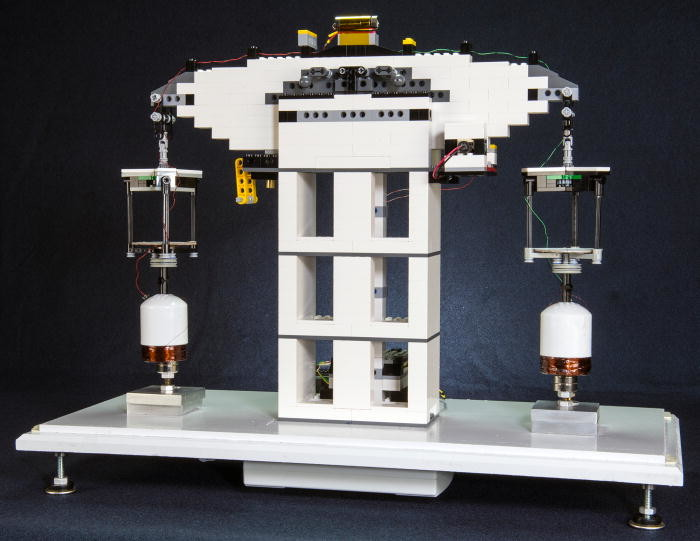
\includegraphics[width=.95\linewidth]{figs/Lego_ Watt_Balance.jpeg}
%      \caption{The LEGO Watt balance created by scientists at NIST \cite{Chao2015}. We intend to build our first prototype as a model of this design.}\label{fig:Lego_Watt_Balance}
% \end{figure}

\begin{figure}
    \centering
    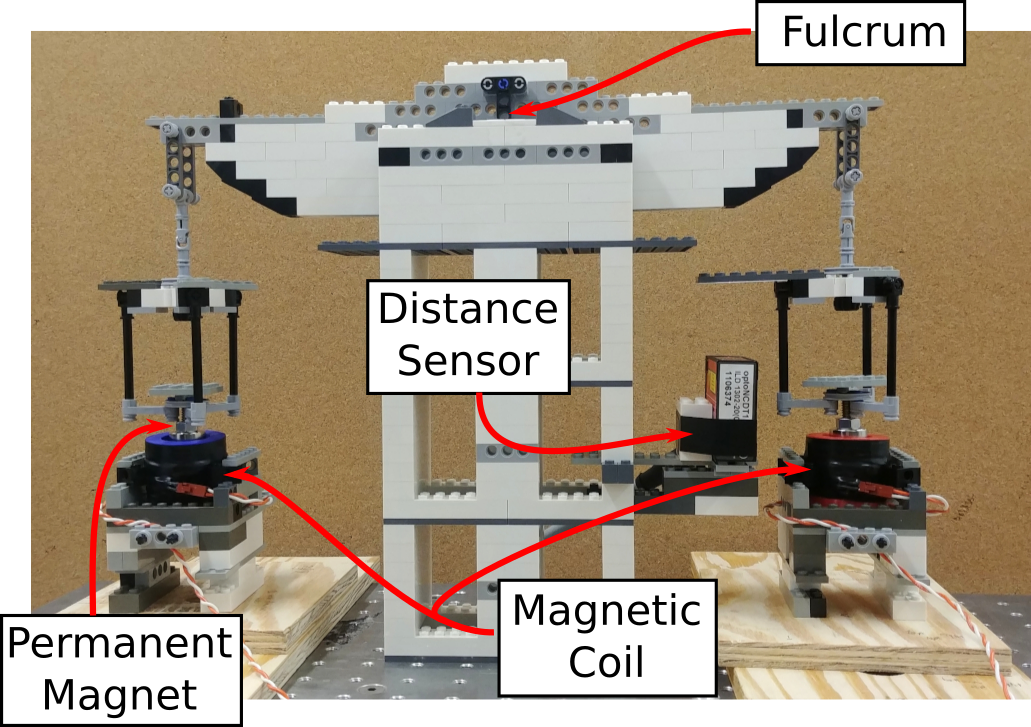
\includegraphics[width=0.95\linewidth]{figs/watt_balance2.jpg.png}
    \caption{Caption}
    \label{fig:our_balance}
\end{figure}

% to redefine the SI Kilogram in terms of Plank's constant.

% We intend to build a Watt balance capable of relating mechanical power to electrical power. The official NIST Watt balance uses the Josephson and quantum Hall effect to measure voltage and current as a function of an irradiating frequency and Planck's constant. The device we build will not be able to rely on these quantum effects for the electrical measurements, meaning that we will not be able to measure Planck's constant. 

% Our experiment will not be able to relate our measu

% Our experiment will be to build a Watt balance capable of balancing mechanical and electrical power. Unlike the official Watt balance at NIST we will not be able to use the Josephson and Hall effects to directly relate our measurements to Planck's constant. Instead we use a peculiarity of electrical unit definitions. Conventional electrical units are based on the conventional values of the Josephson constant $K_{J-90}$ and von Klitzing constant $R_{K-90}$. The 2019 redefinition of SI units fixes the values of these constants exactly, although there is a difference on the order of $1-^{-8}$.








% \begin{figure}[t]
%     \centering\includegraphics[width=.95\linewidth]{fig1.png}
%     \caption{}\label{fig:fig1}
% \end{figure}



\section{Theory}\label{s:theory}

A Watt balance operates by balancing an electromagnetic force with a mechanical force. This can be done by operating the Watt balance in two modes. In the velocity mode one coil is driven to create oscillating motion in the arm while the other coil uses Faradays law to measure an induced electro-motive force $\mathscr{E}$. In the force mode only one coil is operated to provide a force which balances the gravitational force acting on a mass. As mentioned earlier, the velocity mode is a pseudo-calibration step, which will be described in further detail in this section.

% The Watt balance may appear to be similar to an equal-arm balance, however this balance is passive and needs a calibrated mass to compare with the unknown one. A Watt Balance can determine an unknown weight by compensating with a known force, in this case a precisely adjusted electromagnetic force.

% Two modes of measurement are used in this experiment to relate these opposing forces. Both modes, Velocity mode and Force mode, are based on the principle of Lorentz forces. From Faraday’s Law of induction, equation \ref{eq:Faraday}, we know that electromagnetic force is given by the rate of change of magnetic flux through a material.

Faraday's Law states that when a permanent magnet moves near a looped wire, an emf $\mathscr{E}$ is produced, which induces a voltage in the wire proportional to the number of loops $N$ and the rate of change of the magnetic flux $\Phi_B$
\begin{equation}\label{eq:Faraday}
\mathscr{E} =-N\frac{d \Phi_B}{dt}.
\end{equation}

If we assume that the rate of change of the magnetic flux is proportional to the velocity of the permanent magnet, then we can rewrite this equation as follows:
\begin{equation}\label{eq:velocity_equation}
    V=(\Phi_B N)v
\end{equation}

When the balance arm is driven in the velocity mode, a voltage is induced proportional to the magnetic flux $\Phi_B N$ and the velocity of the arm. This measurement can be used to factor out the flux $\Phi_B N$ in the force mode, as will be described below.

% For the Velocity mode measurement, a coil (wire length $L$) is moved at a vertical speed $v$ through a magnetic field (flux density $\Phi_B$) so that a voltage V is induced in the coil. Through the flux integral the voltage can be calculated as:

% \begin{equation}\label{eq:velocity_equation}
%     V={\Phi_B}Lv.
% \end{equation}

The Lorentz force law can be described as follows, where $q$ is a charge, $v$ is its velocity, $E$ is the electric field, and $B$ is the magnetic field:
\begin{equation}
    \vec{F} = q(\vec{E}+v\times \vec{B})
\end{equation}

We can drop the electric field term because the latent electric field is negligible compared to the magnetic field. Expressing the second term in terms of the current $I$ through a length of wire $l$ yields the following:
\begin{equation}
    \vec{F} = I \vec{l}\times \vec{B}
\end{equation}

If the wire is instead looped, then we can integrate this equation over the length of the loop as follows to get a force in the direction normal to the plane of the loop $\hat{n}$:
\begin{equation}
    \vec{F} = I\int\vec{dl}\times\vec{B}  = (\Phi_B N)I \hat{n}
\end{equation}

% In the force mode the Watt balance 


% \end{eq}
% Additionally, in the force mode measurement Lorentz forces can be combined with the definition of electric current to obtain the electromagnetic force on a coil of wire resulting in equation \ref{eq:Laplace}.

% \begin{equation}\label{eq:Laplace}
% F=I{\int{dl}}\times B
% \end{equation}

In the force mode the Watt balance will be operated to generate a force counteracting the gravitational force on a mass $m$ such that:
\begin{equation}\label{eq:force_equation}
    F=(\Phi_B N)I=mg
\end{equation}
where $g$ is the local acceleration due to gravity. The two modes of measurement and their force diagrams are illustrated in figure \ref{fig:Force}. 

\begin{figure}[t]
     \centering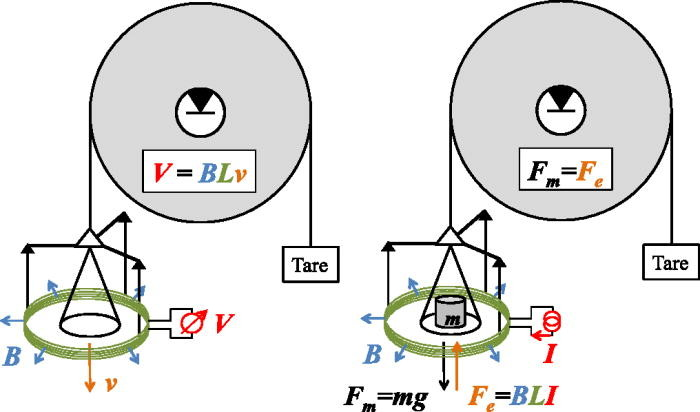
\includegraphics[width=.95\linewidth]{figs/Force_Diagram.jpeg}
     \caption{Velocity mode measurement, illustrated on the left, depicts a coil moving vertically in a radial magnetic field and a voltage $V$ is induced. Force mode measurement, right, displays that the upward electromagnetic force generated by the coil opposes the gravitational force exerted on the mass. \cite{Chao2015}}\label{fig:Force}
\end{figure}

% Mass could be realized simply by using only force mode, however this requires that $(\Phi_B$ and $L$ can be measured accurately. Both of these variables are difficult to measure with enough precision to be usef. 
% Therefore the velocity mode is employed as a calibration method in order for equations \ref{eq:velocity_equation} and \ref{eq:force_equation} to be related independent of the $(\Phi_B N)$ factor. This results in the following equation

Assuming that $(\Phi_B N)$ remains constant between measurements in the velocity and force modes, equations \ref{eq:velocity_equation} and \ref{eq:force_equation} can be used to factor out the $(\Phi_B N)$ term. This is important because the flux $\Phi_B$ is very difficult to measure directly. Furthermore, any linear correction factors that would normally have to be considered in such a setup can be accounted for in the same way as $\Phi_B$. We expect these factors to be present and equal in both modes of operation and can therefore be rolled in with $(\Phi_B N)$. Possible linear correction factors of this sort include the moment of inertia of the balance arm and various linear sources of friction. We arrive at the following equation
\begin{equation}\label{eq:watt_equation}
    VI = mgv
\end{equation}

Equation \ref{eq:watt_equation} relates mechanical power $mgv$ to electrical power $VI$. In our experiment we will measure $V$, $I$, and $v$, assuming $m$ and $g$ are known.
% The goal of this experiment is to compare mechanical power with electrical power using a watt balance.
% and equation \ref{eq:watt_equation}. 
A successful experiment would measure a 1-to-1 correspondence between electrical and mechanical power, confirming equation \ref{eq:watt_equation}. If successful, the watt balance we build could be used to measure other quantities. For example, if the mass of an object is known equation \ref{eq:watt_equation} can be used to measure the local gravitational acceleration. Conversely, if the local gravity is known we can measure the mass of an unknown object.

Finally, we provide an additional discussion on the quantum effects used in the official NIST Watt balance. 
The Josephson effect is an effect in the quantum realm describing current across a Josephson function. A Josephson junction consists of two superconductors coupled by a weak link. when an electric field oscillating at a microwave frequency  $f$ is applied a small current is forced through the junction. This creates a quantized voltage across the junction. Many Josephson junctions can be combined to create a voltage standard that couples the generated voltage to Planck's constant as follows, where $h$ is Planck's constant, $e$ is the charge of an electron, and $K_J$ is Josephson constant
\begin{equation}\label{eq:josephson}
    V=\frac{h}{2e}f \equiv \frac{1}{K_J} f
\end{equation}
The NIST Watt balance uses 250,000 junctions to measure any voltage up to 10\si{V} with a precision of 1\si{nV}. The approximate \$100,000 cost of this setup makes it unfeasable in an MXP classroom setting \cite{Chao2015}.

The quantum Hall effect is a special case of the classical Hall effect, but where the Hall conductance is quantized. This effect occurs in two-dimensional systems of electrons subjected to low temperatures and strong magnetic fields. The quantized Hall conductance $\sigma$ can be described as follows, where $\nu$ belongs to either the set of integers or to a set of known fractions
\begin{equation}
    \sigma = \frac{I}{V_\mathrm{Hall}} = \nu \frac{e^2}{h}
\end{equation}

If we consider only the integer Hall conductance, then we arrive at the following quantized Hall resistance $R_H$, where $R_K$ is the von Klitzing constant
\begin{equation}\label{eq:resistance}
    R_H=\frac{V_H}{I}=\frac{1}{\nu}\frac{h}{e^2} \equiv \frac{1}{\nu} R_K
\end{equation}

The NIST Watt balance uses the quantum Hall effect to measure resistance with a relative uncertainty of 1 in $10^9$. Together with a Josephson voltage standard this can be used to measure current with incredible precision. To determine the value of $VI$ from equation \ref{eq:watt_equation}, we combine two Josephson standards from equation \ref{eq:josephson} and a Hall resistance standard from equation \ref{eq:resistance} to yield the following expression, where $C$ is a known constant related to the number of Josephson junctions
\begin{equation}
    VI=V \frac{V_H}{R_H} = C f_1 f_2 \left(\frac{h}{2e}\right)^2 \frac{e^2}{h}=C \frac{f_1f_2}{4} h
\end{equation}

We see that $h$ finally drops out, and plugging back into equation \ref{eq:watt_equation} yields the following expression
\begin{equation}\label{eq:planck}
    C \frac{f_1f_2}{4} h = mgv
\end{equation}

Equation \ref{eq:planck} defines the kilogram in terms of Planck's constant and other measurements in units defined by other fundamental constants of the universe. This is the desired result.





\section{Experimental Setup}
% \subsection{LEGO Watt Balance Apparatus}

In this section we describe the construction of the Watt balance. The design is based on the Lego Watt balance design illustrated in \cite{Chao2015}, but with some modifications which will be explained below. An image of the completed design is shown in figure \ref{fig:our_balance}.

The design resembles that of a traditional equal arm balance: there is an arm balancing on a small fulcrum with two pans hanging on either side. The pans hang from the balance arm with a universal joint to allow the pans to hang freely. From each pan hangs a brass screw with two neodymium ring magnets mounted. The magnets are oriented such that the magnetic dipoles are aligned anti-parallel. Beneath each magnet pair there is a coil of wire. The coils are 3,000 turns of 36-AWG wire wound around plastic 3D-printed cylinders. The coils are positioned below the magnets with about 10\si{mm} clearance. Increasing the clearance lifts the magnets out of the coils. This gives the balance arm a larger range of motion, but will decrease the magnitude of the magnetic flux through the coils.

Both the force mode and velocity mode require knowing the displacement of the magnets from the balanced position. For this purpose a compact laser triangulation displacement sensor, specifically a Micro-Epsilon optoNCDT ILD1302, is used. This sensor has a measurement range of 30mm to 50mm. 
% TODO resolution of micro epsilon?
The sensor is attached to the base of the device and oriented to point at a bar extending from one of the pans. The device is positioned so the range of motion of the arm falls within the measurement range of the device. The device determines the position of the arm by reflecting a laser off the bar. A smooth piece of paper is glued to the bottom of the bar to ensure the laser reflects uniformly from the surface.

One coil is connected to an HP Agiletn 33120A function generator, which is controlled by a LabView program. This coils is only driven in the velocity mode. The other coil is connected to two different devices depending on the mode of operation. In the velocity mode we measure the current through the coil, while in the force mode the coil is driven with a steady current. In both modes this coil is connected to a data acquisition card (DAQ).
% TODO determine what daq card we're using
To protect the DAQ from the large load of the coil an amplifier is connected between the DAQ and the coil for the force mode.
% TODO determine what amplifier we are using

% TODO explain why the coils are positioned below instead of above
Previous work in building a Lego based Watt balance \cite{Chao2015} had the permanent magnets mounted below with the coils hanging from the pans. Such a design would have wires running from the coils up past the pans to the arm, then to the center of the arm, then down through the center of the base. We found that these wires were stiff enough to apply a torque at two locations. Both the balance of the arm as well as the balance of the pans below the arm were affected. We instead decided to hang the permanent magnets from the pans and place the coils on the ground. The permanent magnets are significantly heavier than the coils, so such a configuration significantly increases the moment of inertia of the balance. 
% TODO do we need to add a sentence at the end of this? To say why it's ok to swap the magnets and the coils



% We intend to build a watt balance based loosely on the LEGO based design described in \cite{Chao2015}, and illustrated in figures \ref{fig:Lego_Watt_Balance} and \ref{fig:chao_balance}. The device resembles a traditional balance beam in its construction, but there is only a platform on one side, and electromagnetic coils hang from both sides. The magnetic system will consist of two neodymium (N48) ring magnets per coil. We intend to maintain the "yokeless" design described in \cite{Chao2015} in order to ensure that the magnetic flux does not deviate from the radial direction. These ring magnets will fit within the PVC pipe coils illustrated in figure \ref{fig:chao_balance} with approximately $0.5\si{cm}$ clearance all around the magnets. A brass threaded rod will be secured to a non-magnetic base plate providing the vertical guide for each magnet system. The magnets will be mounted on the brass rod such that they repel each other with two aluminum nuts on either side of magnets to set their separation distance. This design allows us to alter the position of the magnets and the geometrical center of the entire magnet assembly. 

% \begin{figure}[t]
%     \centering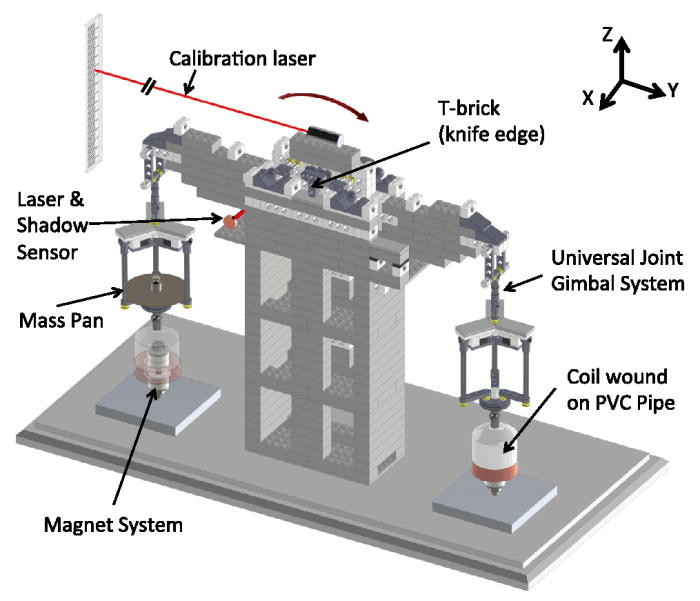
\includegraphics[width=.95\linewidth]{figs/paper_diagram.jpg}
%     \caption{A computer model of the Watt balance designed by Chao et al. \cite{Chao2015}. The balance pivots about the center T-block. Two PVC end caps with copper windings hang from universal joints off either side of the balance beam creating coil A (Left) and coil B (Right). A 10\si{g} mass sits on a mass pan located over coil A, and each coil is concentric to its own magnet system. Two lasers are used to calibrate the system and to measure linear velocity.}\label{fig:chao_balance}
% \end{figure}

% Each coil will be made by designing and 3D printing two cylinders, similar to the ones used in figure \ref{fig:Lego_Watt_Balance}. This method was chosen as it is nonmagnetic, inexpensive, and relatively easy to create with access to the appropriate equipment. The coils will be created using AWG-36 wire about 3000 windings. Increasing the number of windings will result in a larger vertical electromagnetic force and, hence, a larger $BL$ factor. A small hole will be drilled into each cylinder where a LEGO cross axle will be attached allowing each coil to hang rigidly beneath their respective mass pan. 

% The mass pan will be suspended from three rigid rods linking to a LEGO universal joint. A dual-gimbal system will be created and hangs from a set of two freely pivoting axles parallel to the central pivot point on the balance arm. The central pivot has a "knife edge" of approximately 3.1 \si{mm} in the design illustrated in figure \ref{fig:chao_balance}. We intended to imitate this design, however this knife edge can be reduced to increase the sensitivity of the balance. %Printing or laser cutting a new pivot point may improve the resolution of the balance for our design.

%Additionally, we intend to remove the laser pointer/shadow sensor setup in favor of a Microepsilon optical detector, described in \cite{epsilon}, to measure the velocity. This device can measure position to a much higher precision and allows the reading to be interfaced directly with a computer. We intended to mount this device to the balance arm similar to the laser pointer. 

\section{Data Collection Process}

% The data collection process will involve multiple steps before a relation of mechanical and electrical power can be made.
% The two measurements modes, velocity and force, are required for this relation and are measured in different ways. LabVIEW programs and an A2D card will be used to collect the data for both measurements.

In this section we describe the data acquisition process. In the first stage the emf induced in the loop is measured as a function of the velocity of the balance arm. In the second stage the current required to balance the arm is measured for a given mass configuration. We begin by describing the data acquisition process for the velocity mode.

\subsection{Velocity Mode Measurement}

Both coils are used in the velocity mode measurement. In this section Coil A refers to the coil where the induced emf is measured, while Coil B refers to the coil being driven. Coil B is driven by the function generator with a sinusoidal wave with frequency $500\si{Hz}$ and amplitude $0.5V_{pp}$. The natural frequency of the balance arm was found to be near 650Hz. The coil is driven near the natural frequency but not quite at the same value.
% TODO why^

Driving Coil B oscillates the permanent magnets in and out of coil A. This induces an emf in coil A proportional and in phase with the velocity of the oscillatory motion. While Coil B is driven, the micro-epsilon sensor measures the position of the bar over time while the DAQ measures the amplitude of the induced emf over time. The LabView program running the data acquisition program ensures that the position and emf measurements are synchronized to within a few milliseconds. A time step of $10\si{ms}$ is used for both measurements. The velocity is determined from the position data by calculating the symmetric difference quotient of the position data with respect to time. The constant of proportionality between the velocity $v$ and emf $\mathscr{E}$ gives the desired quantity of the magnetic flux $\Phi_B N$. This can be determined from the measurements using a linear least squares regression.

% The velocity mode measurement of $(\Phi_B N)_v$ is crucial to measuring the electromagnetic properties of the balance. The method we will use involves measuring the displacement of the balance arm as one coil is driven with a predetermined sinusoidal signal, from a function generator, to induce a voltage. For this measurement we will utilize the Microepsilon detector to measure the change in position of the balance arm. This device has a measuring range of approximately twenty millimeters and will be mounted to the base of the apparatus under one side of the balance arm. We will then plot the coils velocity against the induced voltage and, using a fitting algorithm, calculate the slope of the curve generated which is equal to $(\Phi_B N)_v$. 

\subsection{Force Mode Measurement}

This measurement involves placing a known mass onto the mass pan, located above coil A in figure \ref{fig:chao_balance}, and inducing an electromagnetic force on coil B to counteract the gravitational force of the mass. The magnitude of the electromagnetic force will be controlled in a way such that the balance arm will stay in it's nulled position after masses are added or removed. A proportional integral derivative controller (PID), programmed using LabVIEW, will be used to regulate the electromagnetic force. This type of controller uses manual feedback to automate the changes necessary in the
electromagnetic force to hold the balance in the null position. Several constants will need to be determined and inputted into the PID controller to regulate this specific system.

The measurement process will involve measuring the current needed to balance a tare mass and a calibrated mass. We can then relate the two measurements to solve for the $(\Phi_B N)_F$ factor. However, to cancel out any drift that may occur in our measurements of current the measurement process will be repeated multiple times with the same masses. This will improve the accuracy of calculated $(\Phi_B N)_F$ factor. In order to calculate the flux integral from force mode, we need to know the local gravitational constant $g$ which can be referenced from the National Oceanic and Atmospheric Administration.

% \subsection{Relation of Mechanical and Electrical Power}

% If successful, our watt balance will measure a 1-to-1 correspondence between $(\Phi_B N)_v$ and $(\Phi_B N)_F$. 

\newpage

 

% \newpage
% \nocite{lab_manual}
% \section{References}
\bibliography{sources}


% \onecolumngrid
% \newpage
% \begin{appendices}

% \section{Spectrum Analyzer 14.1.1}\label{apx:block-diagram-14.1.1}

% \appendixpdf{Embedded Microprocessor}{1042_source.pdf}{apx:1042_verilog}
% \end{appendices}


\end{document}
